\chapter{User Manual}
\label{sec:userManual}
\section{Starting up the app}
After you have installed Wattitude on your phone, as explained in chapter~\ref{sec:installWattitudePhone}, you can start using the app. 

Firstly, since this version of the app does not have support for directly connecting the app to power measuring devices in your home, you need to add data. This involves adding all the different devices you want to collect usage for and their usage. The usage of a device is added for each day, and if you do not know your past usage, it is possible to add an average usage. This may be found on a note by the power connector on the device.

\subsection{Logging on to Facebook}
Logging on to Facebook is done by entering the "login" option in the drawer meny. This will show a log in window where you need to enter your username and password. Then press the "Log In" button. This log in window is displayed in figure~\ref{fig:fblogin}

\begin{figure}[H]
\centering
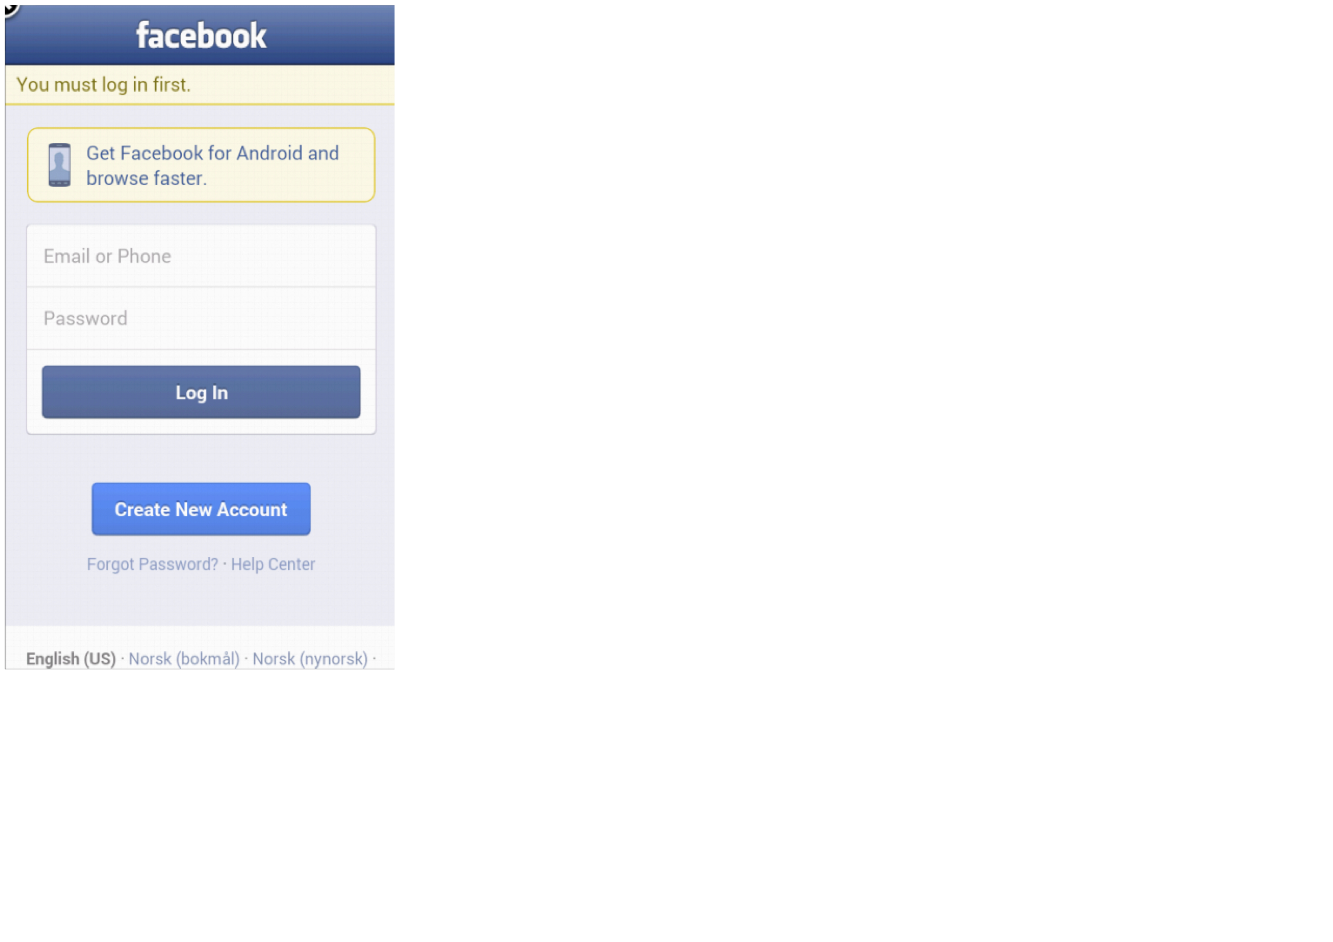
\includegraphics[width=0.5\textwidth, clip, trim=0cm 5.5cm 20.5cm 0cm]{appendix/usermanual/fig/Facebooklogin.png}
\caption{Screenshot of the Facebook login screen}
\label{fig:fblogin}
\end{figure}

\newpage
\section{Devices}
\label{sec:devices}
The device tab includes a collection of all your devices, sorted by their category. In this tab you can manage all of your devices. This include adding new devices, editing the devices you have and deleting your devices. 

\subsection{Adding a new device}
To add a new device press the ''Add devices'' symbol in the option menu. This will make a dialog appear, displayed in figure~\ref{fig:addDevice}. Add the name of the device you want to add and what category the device falls under. You may also add a description of the device.


\begin{figure}[H]
\centering
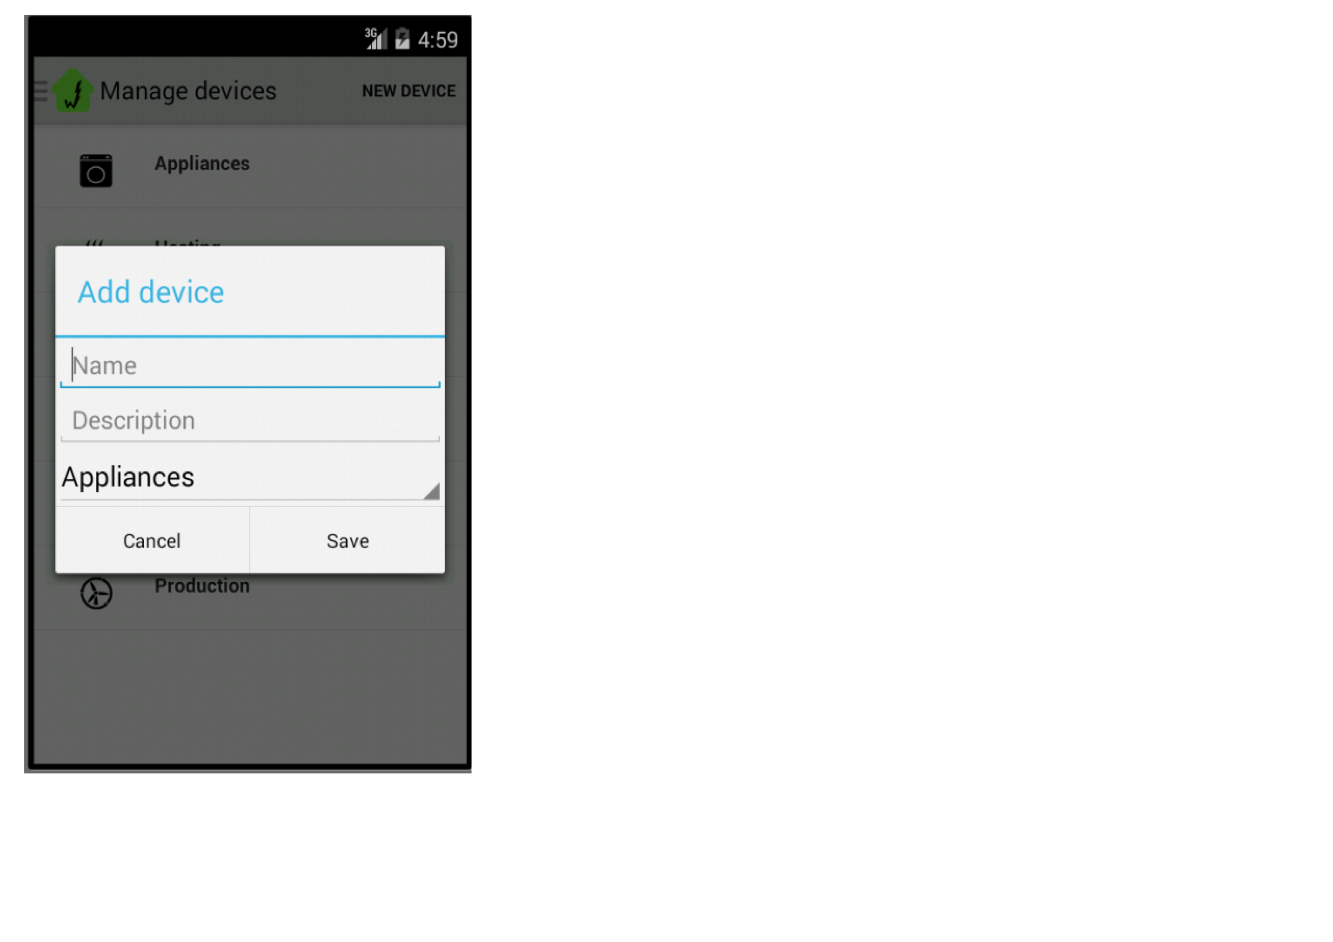
\includegraphics[width=0.5\textwidth, clip, trim=0cm 4cm 19cm 0cm]{appendix/usermanual/fig/AddDeviceDialog.png}
\caption{Screenshot of add device-dialog}
\label{fig:addDevice}
\end{figure}

\subsection{Editing a device}
To modify a device already added to your list of devices, it is necessary to select the device you want to modify. This is done by holding your finger over it. This results in a dialog that gives you the option to edit or delete the device you selected, displayed in figure~\ref{fig:editDevice}. Tap the ''Edit'' button and a new dialog will appear. Enter the new values you want to save to the device you chose.

\begin{figure}[H]
\centering
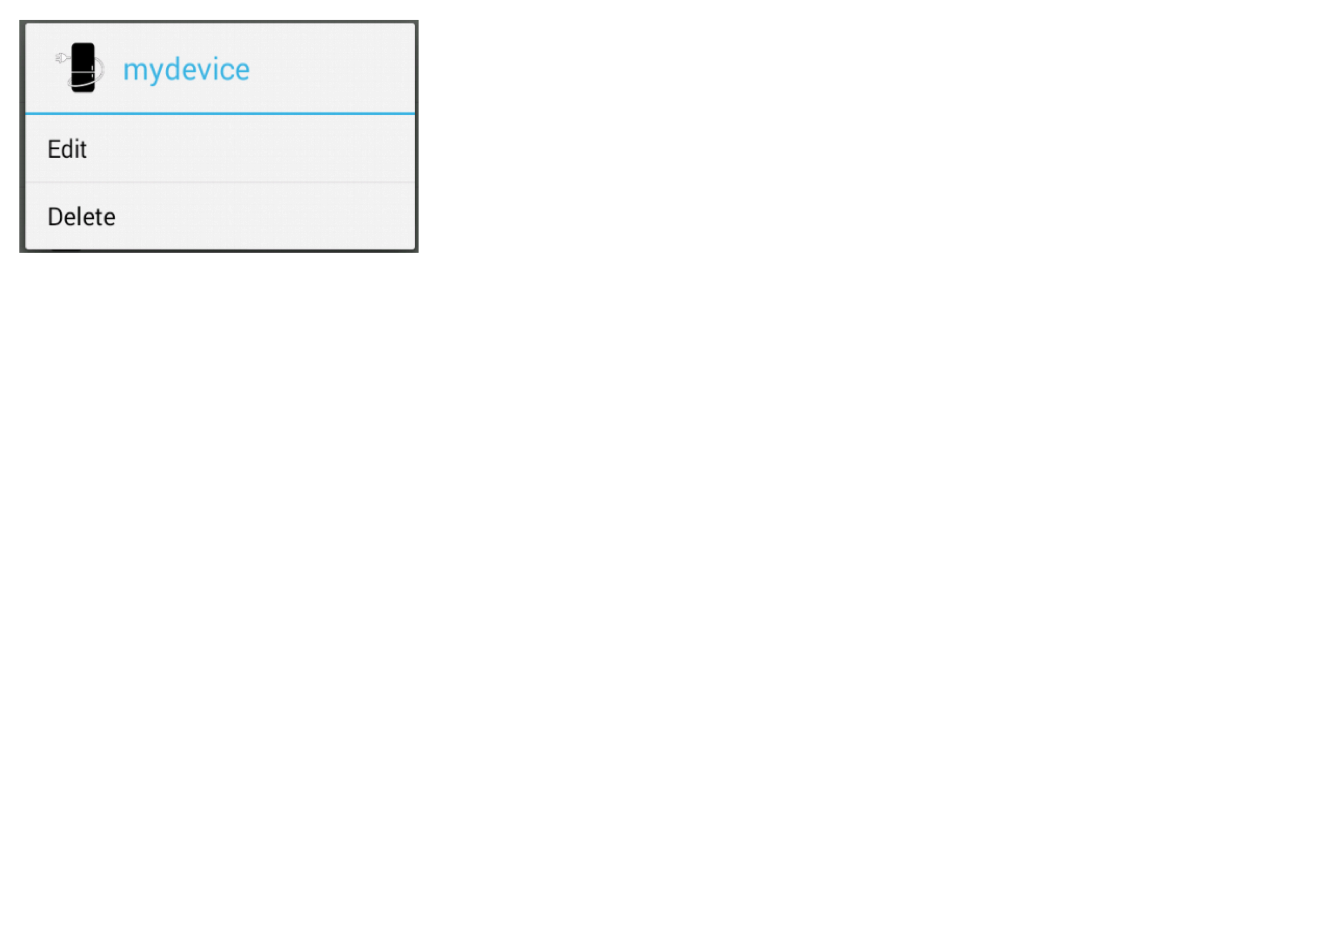
\includegraphics[width=0.5\textwidth, clip, trim=0cm 15cm 20cm 0cm]{appendix/usermanual/fig/EditDeviceDialog.png}
\caption{Screenshot of choose-dialog with edit and delete}
\label{fig:editDevice}
\end{figure}

\subsection{Deleting a device}
To delete a device in your list of devices and press the device you want to delete. Then select ''Delete'' in the dialog that appears. A dialog asking if you really want to delete the device will show, displayed in figure~\ref{fig:deleteDevice}. Press ''OK'', and you will have deleted your device.

\begin{figure}[H]
\centering
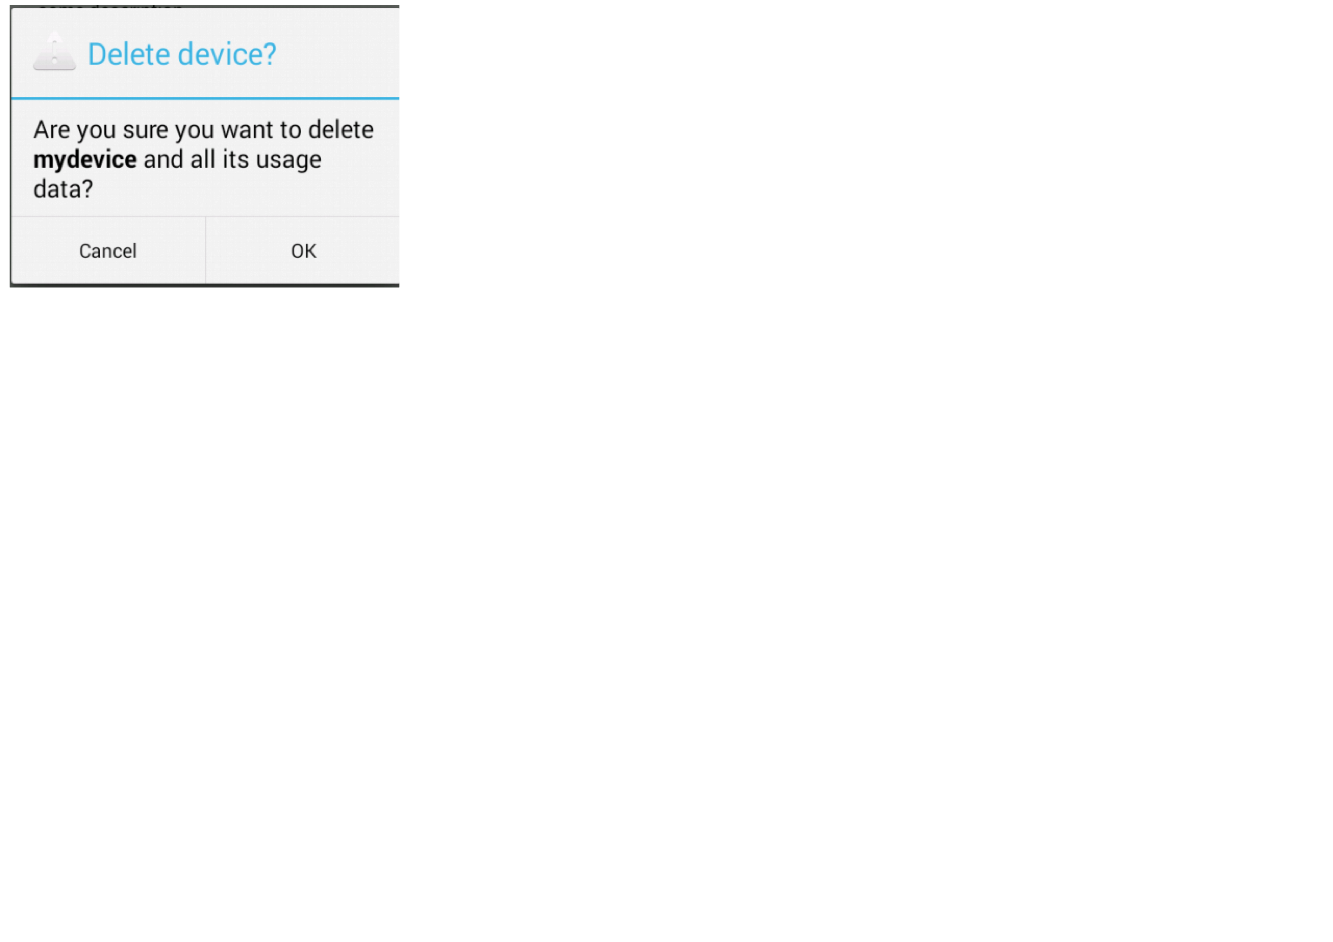
\includegraphics[width=0.5\textwidth, clip, trim=0cm 14cm 20cm 0cm]{appendix/usermanual/fig/ReallyDeleteDevice.png}
\caption{Screenshot of delete-dialog}
\label{fig:deleteDevice}
\end{figure}

\section{Usage}
The usage tab will give you an overview of your usage. You can see the usage of one or several devices, or you can see your total usage. Here, you can also share your usage with your Facebook friends.
\subsection{Adding usage}
To add usage to a device, it is important to first have created a device to add usage to. How to do that is described in section~\ref{sec:devices}. Add usage to your device by selecting the device from the drop down list, pick a date, the amount of energy consumed and lastly press the ''Add usage'' button at the bottom of the screen.

\begin{figure}[H]
\centering
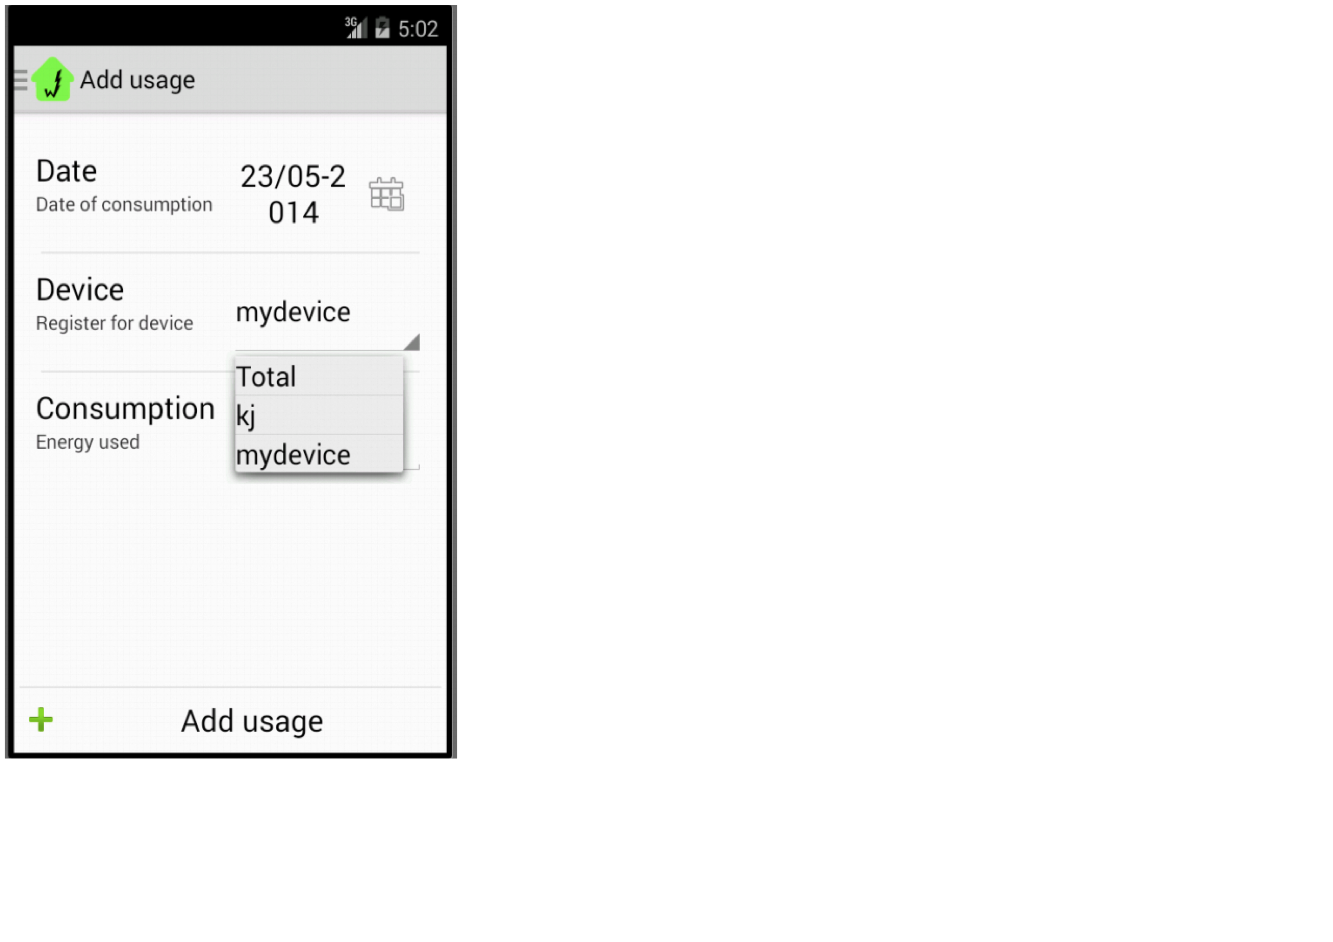
\includegraphics[width=0.5\textwidth, clip, trim=0cm 4cm 19.5cm 0cm]{appendix/usermanual/fig/AddUsage.png}
\caption{Screenshot of adding usage}
\end{figure}

\subsection{Examine your own usage}
You can examine your usage in two different ways. You can look at the usage graph in the usage tab, within the drawer menu user tab. It is also possible to look at how your consumption is distributed between all of your devices. This is done in the distribution tab, within the drawer menu usage tab. 

\begin{figure}[H]
\centering
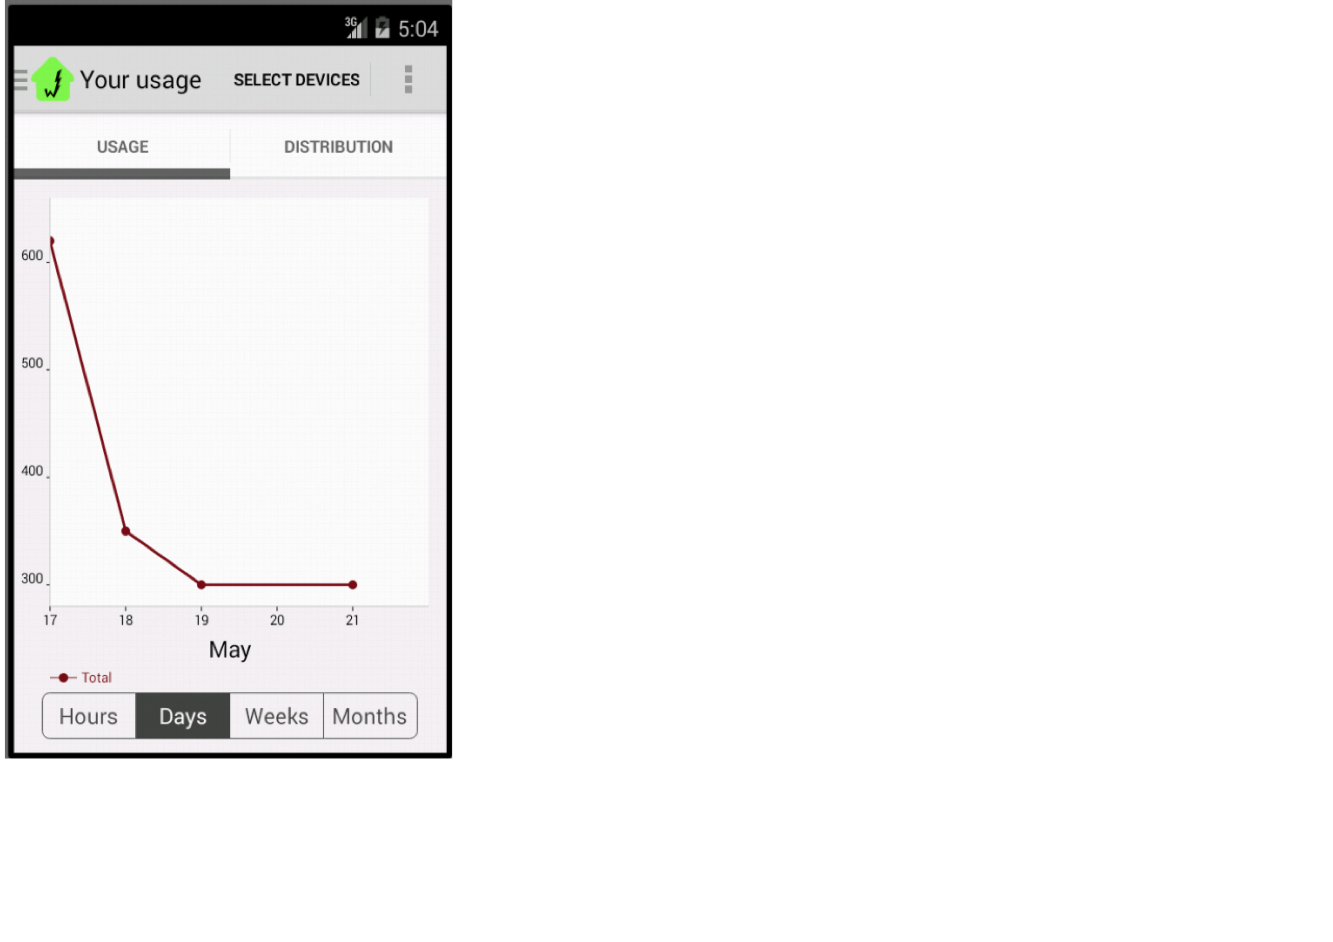
\includegraphics[width=0.5\textwidth, clip, trim=0cm 4cm 19.5cm 0cm]{appendix/usermanual/fig/UsageGraph.png}
\caption{Screenshot of usage graph}
\end{figure}

\newpage
\section{Exchange tips}
Within the exchange tips tab, you can manage all of your tips. Tips is meant to be advise that will help you save energy around your house, when completed.

\subsection{Creating your own tip}
To create your own tip, press the ''Add tips'' button in the option bar. This will create a dialog where you can enter a name of your new tip, and a description.
\subsection{Adding a tip to your list of tips}
Your list of tips is a list of the tips you want to perform in you house. To add a tip to your list of tips, you select the tip you want to add, and a dialog will appear. Select the ''Add to my tip'' option. The tip you added should now appear in the "My tips" tab. 

\begin{figure}[H]
\centering
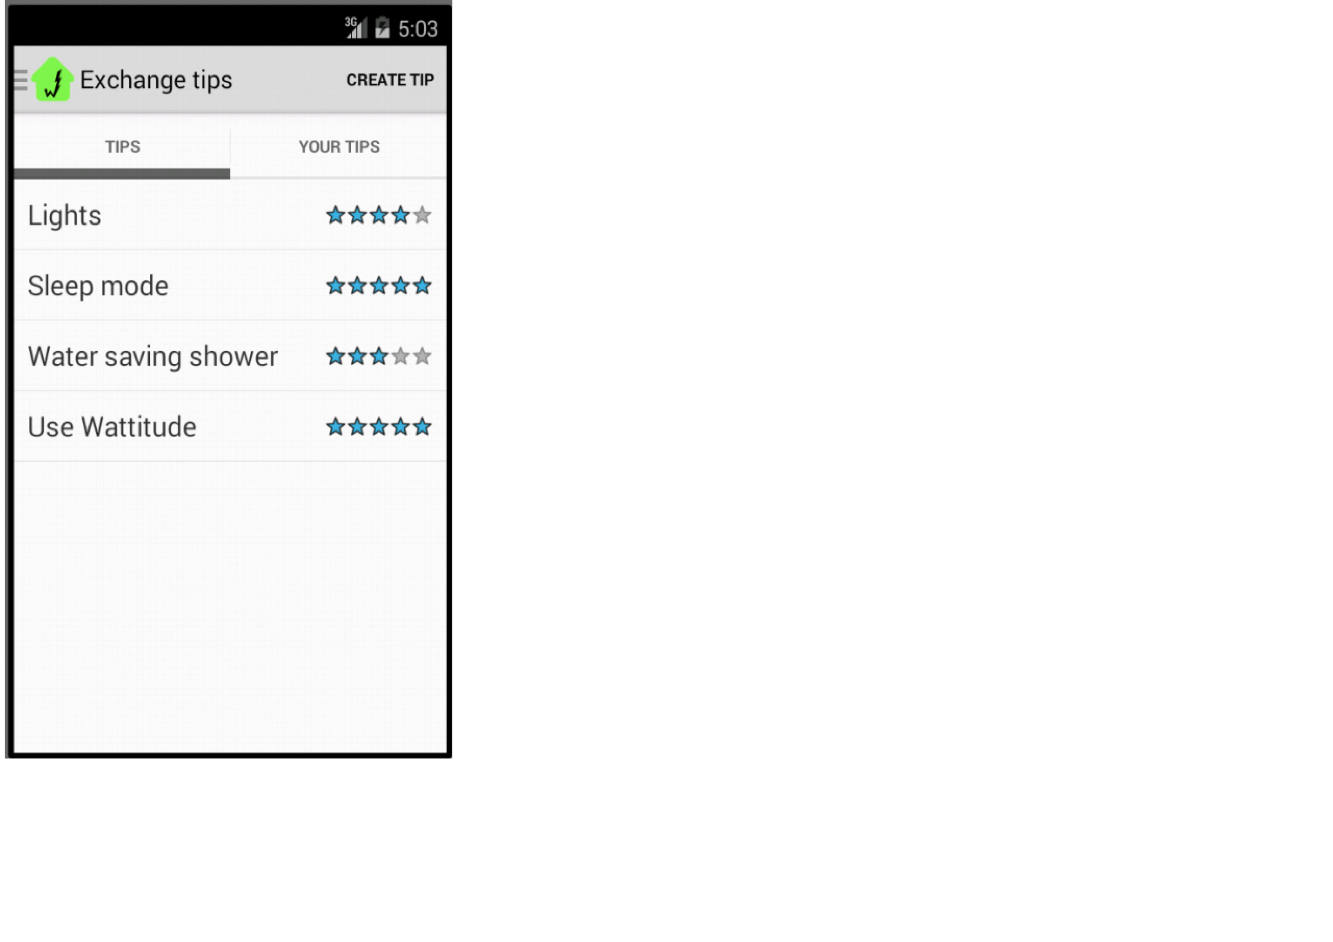
\includegraphics[width=0.4\textwidth, clip, trim=0cm 4cm 19.5cm 0cm]{appendix/usermanual/fig/Tipstab.png}
\caption{Screenshot of list of tips with rating bar}
\end{figure}

\subsection{Indicate that you have performed a tip}
To indicate that you have performed a tip, you check the checkbox beside the tip.
\subsection{Rate a tip}
To change the rating of a tip you hold your finger over the tip you want to change and a dialog will appear. 

